\PassOptionsToPackage{svgnames}{xcolor}
\documentclass[12pt]{article}



\usepackage[margin=1in]{geometry}  
\usepackage{graphicx}             
\usepackage{amsmath}              
\usepackage{amsfonts}              
\usepackage{framed}               
\usepackage{amssymb}
\usepackage{array}
\usepackage{amsthm}
\usepackage[nottoc]{tocbibind}
\usepackage{bm}
\usepackage[object=vectorian]{pgfornament} 
\usepackage{enumitem}
\usepackage{mathtools}
\DeclarePairedDelimiter\ceil{\lceil}{\rceil}
\DeclarePairedDelimiter\floor{\lfloor}{\rfloor}
\colorlet{shadecolor}{lightgray!25}
\newcommand{\sectionline}{%
  \noindent
  \begin{center}
  {\color{DarkViolet}
    \resizebox{0.5\linewidth}{1ex}
    {{%
    {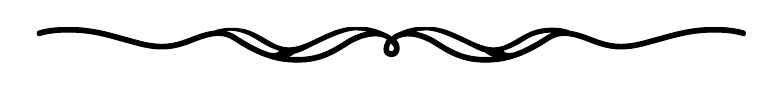
\begin{tikzpicture}
    \node  (C) at (0,0) {};
    \node (D) at (9,0) {};
    \path (C) to [ornament=85] (D);
    \end{tikzpicture}}}}}%
    \end{center}
  }

  \newcommand\norm[1]{\left\lVert#1\right\rVert}
\setlength{\parindent}{0cm}
\setlength{\parskip}{0em}
\newcommand{\Lim}[1]{\raisebox{0.5ex}{\scalebox{0.8}{$\displaystyle \lim_{#1}\;$}}}
\newtheorem{definition}{Definition}[section]
\newtheorem{theorem}{Theorem}[section]
\newtheorem{notation}{Notation}[section]
\theoremstyle{definition}
\DeclareMathOperator{\arcsec}{arcsec}
\DeclareMathOperator{\arccot}{arccot}
\DeclareMathOperator{\arccsc}{arccsc}
\DeclareMathOperator{\spn}{Span}
\DeclareMathOperator{\perm}{P}
\DeclareMathOperator{\combi}{C}
\setcounter{tocdepth}{1}
\begin{document}

\title{Revision notes - MA3269}
\author{Ma Hongqiang}
\maketitle
\tableofcontents

\clearpage
%\twocolumn
\section{Counting}
\subsection{Geometric and Arithmetic Series}
\begin{definition}[Geometric series]
\hfill\\\normalfont A \textbf{geometric series} is a sum of the form
\[
a+ar+ar^2+\cdots+ar^n
\]
\end{definition}
\begin{theorem}[Sum of Geometric series]
\hfill\\\normalfont The value of sum of a geometric series up to $n$th term, $G_n$, for $r\neq 1$, is given by the formula
\[
G_n = a\frac{r^{n+1}-1}{r-1}
\]
\end{theorem}
The following is an example of solving generating functions of an infinite sequence.\\
Suppose $a_0 = 1, a_1 = 1, a_2 = 3$. Also, the recurrence relation of the sequence is $a_n = 2a_{n-1}+1$.
Define the \textbf{generating function} $U(x)$ as follows,

\begin{align*}
U(t)&:=\sum_{n=0}^\infty a_nt^n\;\;\;\;(|t|<1)\\
&=t+\sum_{n=2}^\infty a_nt^n\\
&=t+\sum_{n=2}^\infty (2a_{n-1}+1)t^n\\
&=t+\sum_{n=2}^\infty t^n+2t\sum_{n=2}^\infty a_{n-1}t^{n-1}\\
&=\sum_{n=1}^\infty t^n +2t\sum_{n=1}^\infty a_nt^n\\
&=\sum_{n=0}^\infty t^n-1+2t\sum_{n=0}^\infty a_nt^n\\
&=\sum_{n=0}^\infty t^n-1+2tU(t)\\
&=\frac{1}{1-t}-1+2tU(t)
\end{align*}

Solving $U(t)$ and partial fractioning, we have

\begin{align*}
U(t) &= \frac{1}{1-2t} - \frac{1}{1-t}\\
&=\sum_{n=0}^\infty (2t)^n -\sum_{n=0}^\infty t^n\\
&=\sum_{n=0}^\infty (2^n-1)t^n
\end{align*}

By definition,
\[
U(t)=\sum_{n=0}^\infty a_nt^n = \sum_{n=0}^\infty (2^n-1)t^n
\]
Hence,
\[
a_n = 2^n - 1
\]
\begin{theorem}[Trianglar Number]
\[
T_n = 1+2+3+\cdots+n = \frac{1}{2}n(n+1)
\]
\end{theorem}
\begin{definition}[Arithmetic series]
\hfill\\\normalfont More generally, an \textbf{arithmetic series} is a sum of the form
\[
a+(a+d)+(a+2d)+\cdots+(a+nd)
\]
The number $a$ is called the \textbf{first term} and the number $d$ is called the \textbf{common difference} of the arithmetic series.
\end{definition}
\begin{theorem}[Sum of arithmetic series]
\hfill\\\normalfont The sum of an arithmetic series, up to $n$th term, $A_n$ is given by
\[
A_n = \frac{1}{2}(n+1)(2a+dn)
\]
\end{theorem}
\subsection{Sets}
Similar objects are often gathered together for easy reference. Such a collection is called a \textbf{set}.\\
The item in a set are often referred to as \textbf{elements} or \textbf{members} of the set.\\
We exhibit members of a set within parentheses:
\[
S = \{a,e,i,o,u\}\;\;\;\text{or}\;\;\;S=\{x:x \text{ is a vowel of the English alphabet}\}
\]
We use the notation $x\in S$ to mean "$x$\textit{ is }a member of $S$". \\The notation $x\not\in S$means "$x$ \textit{ is not }a member of $S$".
\begin{definition}[Empty Set]
\hfill\\\normalfont The \textbf{empty set} is the set containing \textit{no} members. This is denoted by $\varnothing$. That is
\[
\varnothing = \{\}
\]
\end{definition}
\begin{definition}[Union]
\hfill\\\normalfont The \textbf{union} of sets $A$ and $B$ is the set whose elements are precisely those belong to $A$ or $B$. Symbolically, we denote the union by $A\cup B$:
\[
A\cup B = \{x:x\in A \text{ or } x\in B\}
\]
\end{definition}
\begin{definition}[Intersection]
\hfill\\\normalfont The \textbf{intersection} of sets $A$ and $B$ is the set whose elements are precisely those belong to $A$ and $B$. Symbolically, we denote the intersection by $A\cap B$:
\[
A\cap B = \{x:x\in A \text{ and } x\in B\}
\]
\end{definition}
\begin{definition}[Disjoint Set]
\hfill\\\normalfont Sets $A$ and $B$ are \textbf{disjoint} if
\[
A\cap B = \varnothing
\]
\end{definition}
\begin{theorem}[Properties of union and intersection]
\hfill\\\normalfont
\begin{itemize}
  \item $A\cup B = B\cup A$, $A\cap B = B\cap A$.
  \item $(A\cup B)\cup C = A\cup(B\cup C)$
  \item $(A\cap B)\cap C = A\cap (B\cap C)$
  \item $A\cup(B\cap C) = (A\cup B)\cap (A\cup C)$
  \item $A\cap(B\cup C) = (A\cap C)\cup (A\cap C)$
  \item $A\cup A = A$, $A\cap A = A$
  \item $A\cup \varnothing = A$, $A\cap \varnothing = \varnothing$
\end{itemize}
\end{theorem}
\begin{definition}[Subset]
\hfill\\\normalfont If every element of $A$ is also an element of $B$, then $A$ is a \textbf{subset} of $B$.
\[
A\subseteq B
\]
\end{definition}
Some immediate consequence of the definition of a subset:
\begin{itemize}
  \item For any set $A$, $A\subseteq A$, $\varnothing\subseteq A$.
  \item For sets $A$, $B$,
  \[
A\subseteq A\cup B, \;\;\;A\cap B \subset A
  \]
  \item If $A\subseteq B$, then
  \[
A\cup B = B,\;\;\; A\cap B = A
  \] 
\end{itemize}
We are often interested in subsets of a fixed reference set called the \textbf{unviersal set}, usually denoted by $U$.
\begin{definition}[Complement]
\hfill\\\normalfont Suppose $U$ is the given universal set, and $A\subseteq U$. Then the \textbf{complement} of $A$, denoted by $A^c$, is the set consisting of all the elements of $U$ which are not in $A$. That is
\[
A^c = \{x\in U: x\not\in A\}
\] 
\end{definition}
By definition,
\[
A\cup A^c = U,\;\;\; A\cap A^c = \varnothing
\]
\begin{theorem}[de Morgan's laws]
\hfill\\\normalfont The following properties hold for set $A$,$B$.
\begin{itemize}
  \item $(A\cup B)^c = A^c\cap B^c$
  \item $(A\cap B)^c = A^c\cup B^c$
\end{itemize}
\end{theorem}
\begin{theorem}[Principle of Inclusion and Exclusion]
\begin{equation*}
\begin{aligned}
P(A_1\cup A_2\cup \cdots\cup A_n)=&\sum_{i=1}^n P(A_i) -\sum_{1\leq i_1\leq i_2\leq n}P(A_{i_1}A_{i_2})+\cdots\\&+(-1)^{r+1}\sum_{1\leq i_1\leq\cdots\leq i_r\leq n}P(A_{i_1}\cdots A_{i_r})\\&+\cdots+(-1)^{n+1}P(A_1\cdots A_n)
\end{aligned}
\end{equation*}
\end{theorem}
\begin{definition}[Floor function]
\hfill\\\normalfont For any real number $x$, the \textbf{floor} of $x$, denoted by
\[
\floor*{x}
\]
is the largest integer $\leq x$.
\end{definition}
\begin{definition}[Ceiling function]
\hfill\\\normalfont For any real number $x$, the \textbf{ceiling} of $x$, denoted by
\[
\ceil*{x}
\]
is the smallest integer $\geq x$.
\end{definition}
\begin{theorem}[Number of multiples]
\hfill\\\normalfont Let $i$ and $n$ be positive integers. The number of multiples of $i$ among the integers $1,2,\ldots, n$ is 
\[
\floor*{\frac{n}{i}}
\]
\end{theorem}
\subsection{Counting Principles}
\begin{theorem}[Addition Principle]
\hfill\\\normalfont If a choice from set $A_i$ can be made in $n_i$ ways for $i = 1,\ldots, m$, then the number of choices from $A_1\cup \cdots\cup A_m$ is
\[
n_1+\cdots+n_m
\]
\textbf{Necessary condition}: The sets $A_1,\ldots,A_m$ are \textbf{pairwise/mutually disjoint}, i.e. $A_i\cap A_j = \varnothing$ for all $i\neq j$.
\end{theorem}
\begin{theorem}[Multiplication Principle]
\hfill\\\normalfont If a task involves a sequence of $m$ steps, where the $i$th step can be completed in $n_i$ ways, then there are
\[
n_1\times \cdots n_m
\]
ways to complete the task.\\
\textbf{Necessary condition:} The ways each step can be completed are \textbf{indepedent} of each other.
\end{theorem}
\subsection{Arrangements and Combinations}
\begin{theorem}
\hfill\\\normalfont Let $^n\perm_k$ be the number of ways of arranging, in a row, $k$ \textit{different} objects taken from $n$ \textit{different} objects. Then
\[
^n\perm_k = \frac{n!}{(n-k)!}
\]
\end{theorem}
\begin{theorem}
\hfill\\\normalfont The number of ways of arranging in a row $n_1$ \textit{identical} objects of Type 1, $n_2$ identical objects of Type 2, $\ldots$, and $n_k$ identical objects of Type $k$, is equal to
\[
\frac{(\sum_{i=1}^kn_i)!}{\prod_{i=1}^kn_i!}
\]
\end{theorem}
\begin{theorem}[Circular Arrangements]
\hfill\\\normalfont The number of ways of arranging $n$ different objects in a circle is
\[
(n-1)!
\]
\end{theorem}
\begin{theorem}
\hfill\\\normalfont Let $^n\combi_k$ denote the number of ways of choosing $k$ objects from a set of $n$ different objects. Then
\[
^n\combi_k = \frac{n!}{k!(n-k)!}
\]
\end{theorem}
Another notation for $^n\combi_k$ is $\binom{n}{k}$.
\begin{theorem}[Simple properties of binomial coefficients]
\hfill\\\normalfont
\begin{itemize}
  \item $\binom{n}{0}=\binom{n}{n}=1$
  \item $\binom{n}{k}=\binom{n}{n-k}$
  \item $\sum_{i = 0}^n\binom{n}{i}=2^n$
\end{itemize}
\end{theorem}
\subsection{Number of Routes on Rectangular Grid}
\begin{theorem}\hfill\\\normalfont On a rectangular grid, the number of routes from $(i,j)$ to $(k,l)$ moving easterly or notherly without back-tracking is
\[
\frac{((k-i)+(l-j))!}{(k-i)!(l-j)!}=\binom{k+l-i-j}{k-i}=\binom{k+l-i-j}{l-j}
\]
\end{theorem}
\subsection{Pigeonhole Principle}
\begin{theorem}[Pigeonhole Principle]\hfill\\\normalfont
Suppose $m$ objects are distributed among $n$ pigeonholes. If $m>n$, then there is at least \textbf{one} pigeonhole with at least \textbf{two} of the distributed objects.
\end{theorem}
\begin{theorem}[Extended Pigeonhole Principle]\hfill\\\normalfont
If $m$ objects are distributed among $n$ pigeonholes and $m>n$, then there will be \textbf{one} pigeonhole which contains \textbf{at least} $\ceil*{\frac{m}{n}}$ objects.
\end{theorem}
\clearpage
\section{Graphing}
\subsection{Introduction}
\begin{definition}[Graph]
\hfill\\\normalfont A \textbf{graph} is a collection of points and lines connecting \textit{some pairs} of the points.\\
The points are called the \textbf{vertices}.\\
The lines joining any the vertices are called \textbf{edges}.
\end{definition}
Two vertices that are joined by an edge are called \textbf{adjacent} vertices.
\begin{definition}[Simple Graph]
\hfill\\\normalfont A graph without loops and multiple edges is called a \textbf{simple graph}.
\end{definition}
\subsection{Basic Technology}
\begin{definition}[Walk]
\hfill\\\normalfont A \textbf{walk} is a sequence of vertices and edges in a graph such that
\begin{itemize}
  \item the sequence alternates between vertices and edges, starting and ending with vertices; and
  \item each edge in the sequence joins the vertices that occur immediately before and after it in the sequence
\end{itemize}
\end{definition}
A walk that starts and ends at \textit{different} vertices is called an \textbf{open walk}.\\
A walk that starts and ends at \textit{the same} vertex is called a \textbf{closed walk}.\\
A walk that contains \textit{no repeated} vertices \textit{and} edges is called a \textbf{path}.
\begin{definition}[Cycle]
\hfill\\\normalfont A \textbf{cycle} in a graph is a \textbf{closed walk} in which the only repitition is the \textbf{first and last} vertex.
\end{definition} 
\begin{definition}[Length]
\hfill\\\normalfont The \textbf{length} of a walk is defined as the number of edges in the walk, including repetitions.
\end{definition}
\begin{definition}[Degree]
\hfill\\\normalfont The \textbf{degree} of a vertex in a graph is the number of edges that occur at that vertex, with every \textit{loop counted as two}.
\end{definition}
\begin{theorem}[Degree Theorem]
\hfill\\\normalfont In any graph, the sum of all the degrees is equal to \textbf{twice} the number of edges.\\In particular, the sum of all the degrees must be even.
\end{theorem}
\begin{definition}[Odd and Even Vertex]
\hfill\\\normalfont An \textbf{odd} vertex is a vertex whose degree is an odd number.\\
An \textbf{even} vertex is a vertex whose degree is an even number.
\end{definition}
\begin{definition}[Minimum and Maximum Degree]
\hfill\\\normalfont In any graph $G$, the symbol $\delta(G)$ represents the \textbf{minimum} degree in $G$; the symbol $\Delta(G)$ represents the maximum degree.
\end{definition}
\subsection{Trees}
\begin{definition}[Trees]
\hfill\\\normalfont A \textbf{tree} is a simple graph that is connected and contains no cycle.
\end{definition}
\begin{definition}[Leaf]
\hfill\\\normalfont A \textbf{leaf} is a vertex of degree 1.
\end{definition}
\begin{theorem}[Leaf Lemma]
\hfill\\\normalfont Every tree with two or more vertices has at least two vertices of degree 1.
\end{theorem}
\begin{theorem}[Tree theorem]
\hfill\\\normalfont Every tree with $n$ vertices has exactly $n-1$ edges.
\end{theorem}
\subsection{Minimal Spanning Trees}
\begin{definition}[Weighted Graphs]
\hfill\\\normalfont A \textbf{weighted graph} is a graph in which each edge has a number associated with it, which we refer to as the \textbf{weight} of that edge.
\end{definition}
\begin{definition}[Subgraph]
\hfill\\\normalfont A \textbf{subgraph} of a graph $G$ is a graph $H$ whose vertices and edges are taken from those of $G$.
\end{definition}
\begin{definition}[Weight of a graph]
\hfill\\\normalfont The \textbf{weight} of a graph $G$ is the sum of weights of all its edges. Symbolically,
\[
w(G) = \sum_{e\text{ edge of }G}w(e)
\]
where $w(e)$ denotes the weight of the edge $e$.
\end{definition}
\begin{definition}[Spanning Tree]
\hfill\\\normalfont A \textbf{spanning tree} of a given graph $G$ is a subgraph $T$ of $G$ which is a tree and it contains \textbf{all} the vertices of $G$.
\end{definition}
\begin{definition}[Minimal Spanning Tree]
\hfill\\\normalfont A \textbf{minimal spanning tree} of $G$ is a spanning tree which has the \textit{minimum weight} among all the spanning trees of $G$.
\end{definition} 
\begin{theorem}[Prim's algorithm]
\hfill\\\normalfont \textbf{Prim's Algorithm} is a procedure for constructing a minimal spanning tree in a given weighted graph:\\
\textbf{Input}: a weighted graph $G$\\
\textbf{Output}: a minimal spanning tree $T$ of $G$\\
\textbf{Algorithm:}
\begin{itemize}
  \item Start with any vertex and select an edge having the minimum weight among all the edges at that vertex
  \item Consider \textit{all} edges that go from each vertex already reached to a new vertex.\\Select one that has \textit{minimum weight}.
  \item Continue until all vertices have been reached.
\end{itemize}
\end{theorem}
\subsection{Euler Walks}
In this section, we allow graphs to contain loops and multiple edges.
\begin{definition}[Directed graph] 
\hfill\\\normalfont A \textbf{directed graph} is a graph in which \textit{every} edge is assigned a direction indicated by an arrow(called a \textbf{directed edge}).
\end{definition}
\begin{definition}[Walk in directed graph]
\hfill\\\normalfont A \textbf{walk} in a directed graph is a sequence of vertices and directed edges such that
\begin{itemize}
  \item the sequence alternates between vertices and directed edges, starting and ending with vertices; and
  \item each directed edge in the sequence joins the vertices that occur immediately before and after it in the sequence \textbf{in the direction} indicated by the arrow of the directed edge.
\end{itemize}
\end{definition}
\begin{definition}[Euler walk]
\hfill\\\normalfont An \textbf{Euler walk} in a graph is a walk that uses every edge in the graph exactly once.\\
A \textbf{closed} Euler walk (also known as \textbf{Euler circuit}) is an Euler walk that starts and ends at the same vertex.\\
An \textbf{open} Euler walk is an Euler walk that starts and ends at different vertices.
\end{definition}
\textbf{Note:} When tracing an Euler walk,
\begin{itemize}
  \item a vertex may be visited more than once
  \item every edge is visited exactly once
  \item the entire graph is traced without lifting the pen
\end{itemize}
\begin{theorem}[Euler Walk Theorem I]
\hfill\\\normalfont A connected \textit{undirected} graph contains a \textit{closed} Euler walk if and only if \textit{every} vertex has \textbf{even} degree. 
\end{theorem} 
\begin{theorem}[Euler Walk Theorem II]
\hfill\\\normalfont A connected \textit{undirected} graph contains an \textit{open} Euler walk starting from vertex $A$ and ending at vertex $B$ if and only if
\begin{itemize}
  \item vertices $A$ and $B$ have odd degree; and
  \item all the other vertices have even degree.
\end{itemize}
\end{theorem}
\begin{theorem}[Euler Walk Theorem I -- directed version]
\hfill\\\normalfont A connected directed graph contains a \textit{closed} Euler walk if and only if for \textit{every} vertex the number of arrows pointing \textbf{in} is \textit{equal} to the number of arrows pointing \textbf{out}.
\end{theorem}
\begin{theorem}[Euler Walk Theorem II -- directed version]
\hfill\\\normalfont A connected directed graph contains an \textit{open} Euler walk starting from vertex $A$ and ending at vertex $B$ if and only if
\begin{itemize}
  \item for vertex $A$, the number of arrows pointing out is exactly one more than the number of arrows pointing in;
  \item for vertex $B$, the number of arrows pointing in is exactly one more than the number of arrows pointing out;
  \item for all other vertices, the number of arrows pointing in is equal to the number of arrows pointing out.
\end{itemize}
\end{theorem}
\fbox{
\begin{minipage}{\textwidth}
  \textbf{An algorithm} to construct an Euler circuit:
  \begin{enumerate}[label = (\arabic*)]
    \item Make sure the graph is connected and all vertices are even.
    \item Start anywhere. Construct a closed walk without repeated edges.
    \item If the closed walk covers all edges, DONE.
    \item If not, construct another closed walk without repeated edges and combine the two to get a bigger closed walk.
    \item Repeat (4) and stop when all edges are used
\end{enumerate}
\end{minipage}
}
\fbox{
  \begin{minipage}{\textwidth}
  \textbf{Chinese Postman Problem}:\\
  Given a connected weighted graph or directed graph $G$, find the shortest circuit that uses each edge in $G$ \textbf{at least once}.
  \end{minipage}
}
\textbf{The simplest case:}
This occurs when every vertex in the graph has even degree, for in this case an Euler
circuit solves the problem. 
\textbf{General case: Vertices of odd degree present}
\begin{enumerate}
  \item List all odd vertices
  \item List all possible pairing of odd vertices
  \item For each pairing, find paths that connect the vertices with the minimum weight. Find the pairings such that the sum of the weights is minimised.
  \item On the original graph, add the edges that have been found in Step 3
  \item The length of an optimal Chinese postman route is the sum of all the edges added to the total found in Step 4
  \item A route corresponding to this minimum weight is an Euler circuit in the graph obtained in Step 5.
\end{enumerate}
\subsection{Vertex Coloring}
\begin{definition}[Proper Vertex Coloring]
\hfill\\\normalfont A \textbf{proper vertex coloring} of a graph is an assignment of a color to each vertex of the graph in such a way that any two vertices that are adjacent have \textit{different} colours.
\end{definition}
\begin{definition}[Minimal Proper Vertex Coloring]\hfill\\\normalfont
We are interested in a proper vertex coloring of a given graph $G$ using the smallest possible number of colors. Such a coloring is called a \textbf{minimal proper vertex coloring} of $G$.\\
The number of colors that occurs in a minimal proper vertex coloring is called the \textbf{chromatic number} of $G$, denoted by
\[
\chi(G)
\]
\end{definition}
\begin{definition}[Complete Graph]
\hfill\\\normalfont The \textbf{complete graph} on $n$ vertices is a graph on $n$ vertices such that any two vertices are joined by an edge. It is denoted by $K_n$.
\end{definition}
\begin{theorem}[Vertex Coloring Theorem]
\hfill\\\normalfont If a graph $G$ contains a complete graph on $n$ vertices, then a proper vertex coloring of $G$ must use at least $n$ colors. Therefore, $\chi(G)\geq n$.
\end{theorem}
\begin{definition}[Cycle Graph]
\hfill\\\normalfont A \textbf{cycle graph} of length $n$ is denoted by $C_n$.
\end{definition}
\begin{theorem}[Vertex Coloring Theorem II]
\hfill\\\normalfont If a graph $G$ contains a cycle graph $C_n$ on $n$ vertices where $n$ is odd, then a proper vertex coloring of $G$ must use at least 3 colours. Therefore, $\chi(G)\geq 3$.
\end{theorem}
\begin{theorem}[Upper bound algorithm for $\chi$]
\hfill\\\normalfont 
\begin{enumerate}
  \item Arrange the degrees of a graph $G$ in decreasing order:
  \[
  d_1\geq d_2\geq d_3\geq \cdots
  \]
  \item Place the integers $1,2,3,\ldots$ directly under these degrees until you reach an integer $k$ such that $k+1>d_{k+1}$.
\end{enumerate}
Then for this graph $G$, we have
\[
\chi(G)\leq k+1
\]
\end{theorem}
\clearpage
\section{Clocking}
\subsection{Parity of integers}
\begin{definition}[Parity]
\hfill\\\normalfont Two integers are said to be of the same \textbf{parity} if they are either both odd or both even.
\end{definition}
\begin{theorem}[Difference of integers of same parity]
\hfill\\\normalfont If two integers are of the same parity, then their difference is an even integer.
\end{theorem}
\subsection{Congreunce Equations}
\begin{definition}
\hfill\\\normalfont Suppose $a$ and $b$ are integers such that their difference is a multiple of a positive integer $n$. Then we write
\[
a\equiv b \pmod n
\]
where $n$ is called the modulus.
\end{definition}
\begin{theorem}[Properties of modulo arithematic]
\hfill\\\normalfont If the remainder of $a$ when divided by $n$ is $r$, then
\[
a\equiv r \pmod n
\]
$a\equiv b pmod n$ if and only if $a$ and $b$ have the same remainder when divided by $n$.\\
If $a\equiv b\pmod n$, then $a\equiv b\pm n\pmod n$.\\
Suppose $a\equiv b\pmod n$, then
\[
ka \equiv kb \pmod n
\]
where $k$ is a integer; and
\[
a^p\equiv b^p\pmod n
\]
where $p$ is a positive integer.\\
Congruences are transitive in a sense that, if $a\equiv b\pmod n$ and $b\equiv c\pmod n$ then
\[
a\equiv c\pmod n
\]
Two congruences with the same modulus can be added to each other or multiplied one by the other.\\Suppose $a\equiv b\pmod n$ and $c\equiv d\pmod n$ then
\begin{align*}
a+c&\equiv b+d\pmod n\\
ac&\equiv bd\pmod n
\end{align*}
\end{theorem}
\begin{theorem}[Congruence mod 9]
\hfill\\\normalfont Let $S$ be the sum of digits of the decimal representation of the positive integer $N$. Then
\[
N\equiv S\pmod 9
\]
\end{theorem}
\begin{theorem}[Checking product]
\hfill\\\normalfont Suppose $A\times B = C$, then
\[
S\times T\equiv U\pmod n
\]
where $S,T,U$ are the sums of digits of $A,B,C$ respectively.
\subsection{Dates and days of the weak}
\end{theoremw}
\end{document}